% Options for packages loaded elsewhere
\PassOptionsToPackage{unicode}{hyperref}
\PassOptionsToPackage{hyphens}{url}
\PassOptionsToPackage{dvipsnames,svgnames*,x11names*}{xcolor}
%
\documentclass[
  12pt,
]{article}
\usepackage{lmodern}
\usepackage{setspace}
\usepackage{amssymb,amsmath}
\usepackage{ifxetex,ifluatex}
\ifnum 0\ifxetex 1\fi\ifluatex 1\fi=0 % if pdftex
  \usepackage[T1]{fontenc}
  \usepackage[utf8]{inputenc}
  \usepackage{textcomp} % provide euro and other symbols
\else % if luatex or xetex
  \usepackage{unicode-math}
  \defaultfontfeatures{Scale=MatchLowercase}
  \defaultfontfeatures[\rmfamily]{Ligatures=TeX,Scale=1}
  \setmainfont[]{Times New Roman}
  \setsansfont[]{Times New Roman}
\fi
% Use upquote if available, for straight quotes in verbatim environments
\IfFileExists{upquote.sty}{\usepackage{upquote}}{}
\IfFileExists{microtype.sty}{% use microtype if available
  \usepackage[]{microtype}
  \UseMicrotypeSet[protrusion]{basicmath} % disable protrusion for tt fonts
}{}
\makeatletter
\@ifundefined{KOMAClassName}{% if non-KOMA class
  \IfFileExists{parskip.sty}{%
    \usepackage{parskip}
  }{% else
    \setlength{\parindent}{0pt}
    \setlength{\parskip}{6pt plus 2pt minus 1pt}}
}{% if KOMA class
  \KOMAoptions{parskip=half}}
\makeatother
\usepackage{xcolor}
\IfFileExists{xurl.sty}{\usepackage{xurl}}{} % add URL line breaks if available
\IfFileExists{bookmark.sty}{\usepackage{bookmark}}{\usepackage{hyperref}}
\hypersetup{
  pdftitle={Emotional framing and the effectiveness of corrective information},
  colorlinks=true,
  linkcolor=Maroon,
  filecolor=Maroon,
  citecolor=Blue,
  urlcolor=Blue,
  pdfcreator={LaTeX via pandoc}}
\urlstyle{same} % disable monospaced font for URLs
\usepackage[margin=1in]{geometry}
\usepackage{longtable,booktabs}
% Correct order of tables after \paragraph or \subparagraph
\usepackage{etoolbox}
\makeatletter
\patchcmd\longtable{\par}{\if@noskipsec\mbox{}\fi\par}{}{}
\makeatother
% Allow footnotes in longtable head/foot
\IfFileExists{footnotehyper.sty}{\usepackage{footnotehyper}}{\usepackage{footnote}}
\makesavenoteenv{longtable}
\usepackage{graphicx,grffile}
\makeatletter
\def\maxwidth{\ifdim\Gin@nat@width>\linewidth\linewidth\else\Gin@nat@width\fi}
\def\maxheight{\ifdim\Gin@nat@height>\textheight\textheight\else\Gin@nat@height\fi}
\makeatother
% Scale images if necessary, so that they will not overflow the page
% margins by default, and it is still possible to overwrite the defaults
% using explicit options in \includegraphics[width, height, ...]{}
\setkeys{Gin}{width=\maxwidth,height=\maxheight,keepaspectratio}
% Set default figure placement to htbp
\makeatletter
\def\fps@figure{htbp}
\makeatother
\setlength{\emergencystretch}{3em} % prevent overfull lines
\providecommand{\tightlist}{%
  \setlength{\itemsep}{0pt}\setlength{\parskip}{0pt}}
\setcounter{secnumdepth}{5}
\usepackage{booktabs}
\usepackage{longtable}
\usepackage{array}
\usepackage{multirow}
\usepackage{wrapfig}
\usepackage{float}
\usepackage{colortbl}
\usepackage{pdflscape}
\usepackage{tabu}
\usepackage{threeparttable}
\usepackage{threeparttablex}
\usepackage[normalem]{ulem}
\usepackage{makecell}
\usepackage{xcolor}

\title{Emotional framing and the effectiveness of corrective information\footnote{I thank Thomas Bräuninger, Sebastian Juhl, the GIP team, and participants of the CDSS workshop in political science for excellent comments and helpful suggestions on this study. This work was supported by the German Research Foundation (DFG) via the Collaborative Research Center (SFB) 884 on ``The Political Economy of Reforms'' (Project C2) and the University of Mannheim's Graduate School of Economics and Social Sciences.}}
\author{Pirmin Stöckle\footnote{Corresponding address: \href{mailto:pirmin.stoeckle@gess.uni-mannheim.de}{\nolinkurl{pirmin.stoeckle@gess.uni-mannheim.de}}}\\
GESS and SFB 884, University of Mannheim}
\date{\today}

\begin{document}
\maketitle
\begin{abstract}
\setstretch{1} \noindent Concerns about various forms of misinformation and its fast dissemination through online media have generated huge interest into ways to effectively correct false claims. An under-explored mechanism in this research is the role of distinct emotions. How do emotional appeals interact with corrective information? Specifically, I focus on the emotion of disgust, which has been shown to be linked to the moralization of attitudes, which in turn reduces the impact of empirical evidence on attitudes and makes compromise less likely. Substantively, I investigate the issue of genetically modified (GM) food. I implement a pre-registered survey experiment within a panel study based on a probability sample of the general population in Germany (N = 4,000). Results show what we have learned about the question. This study provides evidence on the effect of emotionally charged disinformation on perceptions of GM food, and ways to effectively correct false claims. In a broader perspective, these results inform further studies and policy interventions on other issues where disinformation loads on strong emotions, ranging from social policy over immigration to health interventions such as vaccinations. \vspace{.8cm}
\end{abstract}

\setstretch{1.2}
\newpage

\hypertarget{introduction}{%
\section{Introduction}\label{introduction}}

How do emotional appeals interact with corrective information?
Fueled by the fast dissemination through digital media, the issue of various forms of misinformation has become a major concern both in academia and for public policy (Jerit and Zhao \protect\hyperlink{ref-jerit2020political}{2020}; Lazer et al. \protect\hyperlink{ref-lazer2018science}{2018}; Lewandowsky et al. \protect\hyperlink{ref-lewandowsky2012misinformation}{2012}; Wardle and Derakhshan \protect\hyperlink{ref-wardle2017information}{2017}).
To limit the danger from inaccurate or misleading information, efforts of fact-checking or corrective information more generally are widely applied (Walter et al. \protect\hyperlink{ref-walter2020fact}{2020}). A common finding in the maturing literature on corrective information is that these interventions are usually successful in reducing misperceptions, but may not translate to other outcomes such as attitudes, candidate evaluations or blame attribution (Bisgaard \protect\hyperlink{ref-bisgaard2019getting}{2019}; Nyhan et al. \protect\hyperlink{ref-nyhan2019taking}{2019}; Swire-Thompson et al. \protect\hyperlink{ref-swire2019they}{2019}; Thorson \protect\hyperlink{ref-thorson2016belief}{2016}).

While this has been linked to affect (Thorson \protect\hyperlink{ref-thorson2016belief}{2016}), the connection of distinct emotions to both susceptibility to misinformation, and the effectiveness of corrective information is under-explored (exceptions include (Ecker, Lewandowsky, and Apai \protect\hyperlink{ref-ecker2011terrorists}{2011}; Martel, Pennycook, and Rand \protect\hyperlink{ref-martel2020reliance}{2020}; Rosenzweig et al. \protect\hyperlink{ref-rosenzweig2020misinformation}{2020}; Weeks \protect\hyperlink{ref-weeks2015emotions}{2015}). This is unfortunate given the important role that emotional appeals play in the dissemination of false or misleading information. We know that false news spread faster than true news, possibly because they are more likely to evoke emotions of surprise and disgust (Vosoughi, Roy, and Aral \protect\hyperlink{ref-vosoughi2018spread}{2018}). In general, moral-emotional language is rewarded on social media (Brady et al. \protect\hyperlink{ref-brady2017emotion}{2017}) and populist parties use more negative emotional appeals in their communication than non-populist parties (Widmann \protect\hyperlink{ref-widmann2021how}{2021}).

Emotions certainly play an important role in politics (Redlawsk \protect\hyperlink{ref-redlawsk2006feeling}{2006}), and approaches such as cognitive appraisal theory (Moors et al. \protect\hyperlink{ref-moors2013appraisal}{2013}) or affective intelligence theory (Marcus, Neuman, and MacKuen \protect\hyperlink{ref-marcus2000affective}{2000}; Marcus et al. \protect\hyperlink{ref-marcus2019applying}{2019}) provide frameworks for empirical expectaitoins about specific emotions.
In this study, I follow recent work in political science inspired by moral psychology. Most relevant for this study, Clifford (\protect\hyperlink{ref-clifford2019emotional}{2019}) finds that a persuasive emotional frame loading on emotions of anger and disgust increases the perception of an issue as being one of moral conviction (Skitka et al. \protect\hyperlink{ref-skitka2020psychology}{2020}; Wisneski and Skitka \protect\hyperlink{ref-wisneski2017moralization}{2017}).
Moral conviction, i.e.~the conviction that the handling of an issue touches morality and is about fundamental right or wrong, can be seen as a dimension of attitude strength (Skitka, Wisneski, and Brandt \protect\hyperlink{ref-skitka2018attitude}{2018}).
While it is often seen as a binary categorization whether or not an issue is a moral one, there is quite some variation in the extent of moralization within issues (Ryan \protect\hyperlink{ref-ryan2014reconsidering}{2014}) with distinct behavioral consequences, such as an absolute unwillingness to compromise (Ryan \protect\hyperlink{ref-ryan2017no}{2017}) or a tendency to view that issue in absolutist term and to be less likely to be open for information about consequences (Ryan \protect\hyperlink{ref-ryan2019actions}{2019}).

In his study, Clifford shows that disgust-evoking messages can increase moral conviction with its consequences on polarizing attitudes. However, some of the treatment material used in his study comes from a later retracted study linking GMO and cancer. Such a piece of information can be classified as misinformation in the sense of going against ``best available evidence in the public sphere''(Flynn, Nyhan, and Reifler \protect\hyperlink{ref-flynn2017nature}{2017}, 128).
From findings of belief echoes (Thorson \protect\hyperlink{ref-thorson2016belief}{2016}) and affective perseverance (Sherman and Kim \protect\hyperlink{ref-sherman2002affective}{2002}) we might suspect that such emotional effects of frames may persist even in the face of successful factual correction.

This study contributes to the literature of corrective information by linking the concept of belief echoes to the perseverance of specific emotions with related consequences on attitudes. Specifically, it provides evidence on the effect of emotionally charged disinformation on perceptions of GM food, and ways to effectively correct false claims.

The topic of GM feed is particularly suited for this study because it is an issue where science and public opinion diverge considerably, implying a relevant role for corrective information (Diamond, Bernauer, and Mayer \protect\hyperlink{ref-diamond2020does}{2020}, hasell2020differential, carnahan2019processing). This is especially true within the German population, which is where this study draws its sample from (Gaskell et al. \protect\hyperlink{ref-gaskell2010europeans}{2010}). GM food is also a topic on which there are misperceptions, possibly due to disinformation. Of course, there is legitimate criticism on the use of genetic modification. However, studies show that extreme opponents of GM food know the least about it (Fernbach et al. \protect\hyperlink{ref-fernbach2019extreme}{2019}), and a lack of acceptance of novel food technologies against scientific evidence can be seen as as a threat for the development of a more resilient food system (Siegrist and Hartmann \protect\hyperlink{ref-siegrist2020consumer}{2020}).

In the view of many scientists (Roberts \protect\hyperlink{ref-roberts2018nobel}{2018}, planck2019scientists), genetic engineering provides avenues with large potential benefits, which may be impeded by public resistance possibly originating from misleading claims easily disseminated through online media.
In a broader perspective, these results inform further studies and policy interventions on other issues where disinformation loads on strong emotions, ranging from social policy over immigration to health interventions such as vaccinations.

\hypertarget{theory}{%
\section{Theory}\label{theory}}

\hypertarget{misinformation-and-corrective-information}{%
\subsection{Misinformation and corrective information}\label{misinformation-and-corrective-information}}

Factual beliefs are affected in the direction of presented evidence for both (a) misinformation and (b) corrective information.

The effects on related opinions are much less clear.
Some studies find effects, some not.

Affective responses are at least implicitly discussed in this literature, but discrete emotions are widely neglected.

\hypertarget{emotions-and-political-learning}{%
\subsection{Emotions and political learning}\label{emotions-and-political-learning}}

Although there is a rich literature on emotions in politics shedding light on its effect on information processing, political learning and participation, the connection of distinct emotions to both susceptibility to misinformation and the effectiveness of corrective information is under-explored.

Research has shown that\ldots{} anger\ldots{} anxiety\ldots{} enthusiasms\ldots{}

A recently growing interest is in disgust.
Connection to morality, relevant for immigration, homeless \ldots{}

A study has shown that moral shock works to moralize attitudes towards GM food.
However, the main part of the material used there can be classified as misinformation
GM food is an issue on which disinformation exists. This does not mean that there can or should be no criticism, but concrete adverse health effects are not warranted by evidence. Least knowledgeable people are the fiercest opponents. So

\hypertarget{hypotheses}{%
\subsection{Hypotheses}\label{hypotheses}}

From findings on moral conviction and how emotional frames induce it (Clifford \protect\hyperlink{ref-clifford2019emotional}{2019}; Wisneski and Skitka \protect\hyperlink{ref-wisneski2017moralization}{2017}), I expect that a persuasive message evoking negative emotions, notably disgust and anger, can increase perceptions of the respective issue as being one of moral conviction. In order to count as a persuasive message, I expect the message to affect both factual beliefs and policy opinions in its direction.

\begin{itemize}
\tightlist
\item
  H1 A persuasive, emotionally framed message evoking negative emotions of disgust and anger makes individuals more likely to favor policy restrictions on the respective issue and to perceive the issue as one of moral conviction.
\end{itemize}

Concerning the impact of corrective information, I expect that it will be effective in reducing factual misperceptions, irrespective of the presence of evoked emotions. This is in line with previous research showing no moderation effect on corrections due to emotional framing (Ecker, Lewandowsky, and Apai \protect\hyperlink{ref-ecker2011terrorists}{2011}).

\begin{itemize}
\tightlist
\item
  H2a Corrective information is effective in eliminating the misinformation effect on factual beliefs.
\end{itemize}

However, similar to previous results on affective perseverance (Sherman and Kim \protect\hyperlink{ref-sherman2002affective}{2002}) and belief echoes (Thorson \protect\hyperlink{ref-thorson2016belief}{2016}), I expect the effects of emotionally framed misinformation on policy opinion, moral conviction, and emotions to persist even in the face of effective factual correction.

\begin{itemize}
\tightlist
\item
  H2b The emotionally framed misinformation leaves an impact on policy opinions, moral conviction, and emotions.
\end{itemize}

Together, hypotheses 2a and 2b represent the existence of a ``belief echo'', i.e.~the continued effect of a piece of misinformation on attitudinal or emotional outcomes, despite successful factual correction. If only H2a is supported, the correction is altogether successful.

Corrective information such as fact-checking is usually deliberately presented in a rather neutral way. In the case of strongly emotional framed misinformation, such a neutral correction may thus be successful in correcting factual beliefs, but not be able to counter the emotional impact of the misinformation. If this is the case, a more effective strategy may be to counter the emotional misinformation not with a neutral correction but with a correction embedded in an emotional counter-frame. If equally persuasive, such counterframes have been shown to negate the effect of an original frame (Chong and Druckman \protect\hyperlink{ref-chong2013counterframing}{2013}). I expect a similar effect to hold in response to emotionally framed misinformation.

\begin{itemize}
\tightlist
\item
  H3 A correction embedded in a persuasive emotional counter-frame eliminates the misinformation effect on policy opinions, moral conviction, and emotions.
\end{itemize}

\hypertarget{gmo---a-case-for-emotional-reactions-and-misinformation}{%
\subsection{GMO - a case for emotional reactions and misinformation}\label{gmo---a-case-for-emotional-reactions-and-misinformation}}

\hypertarget{data-methods}{%
\section{Data \& Methods}\label{data-methods}}

\hypertarget{results}{%
\section{Results}\label{results}}

\hypertarget{descriptives}{%
\subsection{Descriptives}\label{descriptives}}

\begin{table}
\centering
\begin{tabular}[t]{lrrrrrrr>{}r}
\toprule
  & Unique (\#) & Missing (\%) & Mean & SD & Min & Median & Max &   \\
\midrule
Anger & 5 & 0 & 1.7 & 1.4 & 0.0 & 2.0 & 4.0 & 
\includegraphics[width=0.67in, height=0.17in]{C:/Users/pstoeckl/Documents/GitHub_Projects/emotions-corrective-information/paper_files/figure-latex/hist_2214ac55bc6.pdf}\\
Anxiety & 5 & 0 & 2.4 & 1.2 & 0.0 & 3.0 & 4.0 & 
\includegraphics[width=0.67in, height=0.17in]{C:/Users/pstoeckl/Documents/GitHub_Projects/emotions-corrective-information/paper_files/figure-latex/hist_22147c85086.pdf}\\
Disgust & 5 & 0 & 1.5 & 1.3 & 0.0 & 1.0 & 4.0 & 
\includegraphics[width=0.67in, height=0.17in]{C:/Users/pstoeckl/Documents/GitHub_Projects/emotions-corrective-information/paper_files/figure-latex/hist_22147726477d.pdf}\\
Sadness & 5 & 0 & 1.7 & 1.3 & 0.0 & 2.0 & 4.0 & 
\includegraphics[width=0.67in, height=0.17in]{C:/Users/pstoeckl/Documents/GitHub_Projects/emotions-corrective-information/paper_files/figure-latex/hist_221427ce1c39.pdf}\\
Belief GMO safety & 8 & 0 & 3.2 & 1.6 & 1.0 & 3.0 & 7.0 & 
\includegraphics[width=0.67in, height=0.17in]{C:/Users/pstoeckl/Documents/GitHub_Projects/emotions-corrective-information/paper_files/figure-latex/hist_2214d7d1cfe.pdf}\\
Policy restrictions & 8 & 1 & 5.2 & 1.6 & 1.0 & 5.0 & 7.0 & 
\includegraphics[width=0.67in, height=0.17in]{C:/Users/pstoeckl/Documents/GitHub_Projects/emotions-corrective-information/paper_files/figure-latex/hist_221475322953.pdf}\\
Moral conviction & 10 & 1 & 4.4 & 2.0 & 0.0 & 4.0 & 8.0 & 
\includegraphics[width=0.67in, height=0.17in]{C:/Users/pstoeckl/Documents/GitHub_Projects/emotions-corrective-information/paper_files/figure-latex/hist_22145de319c0.pdf}\\
\bottomrule
\end{tabular}
\end{table}

\hypertarget{moralization}{%
\subsection{Moralization}\label{moralization}}

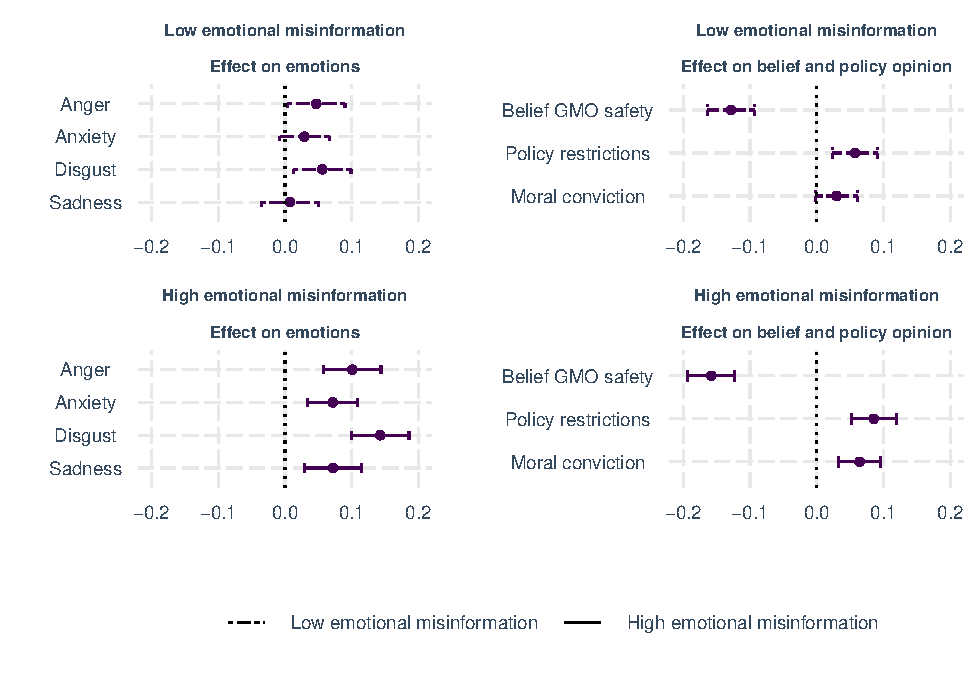
\includegraphics{paper_files/figure-latex/unnamed-chunk-5-1.pdf}

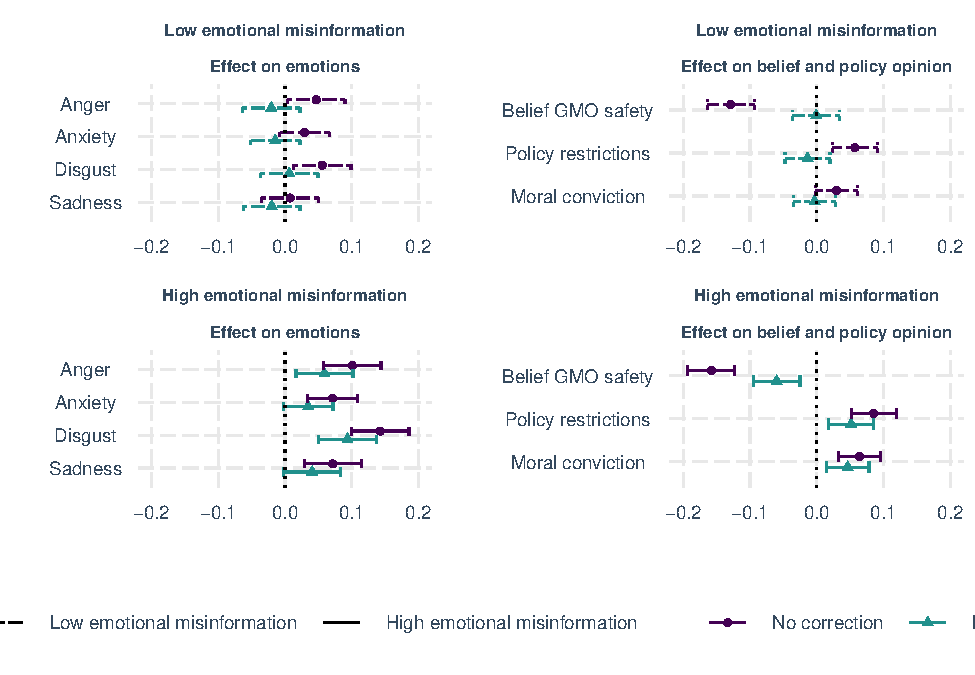
\includegraphics{paper_files/figure-latex/unnamed-chunk-6-1.pdf} 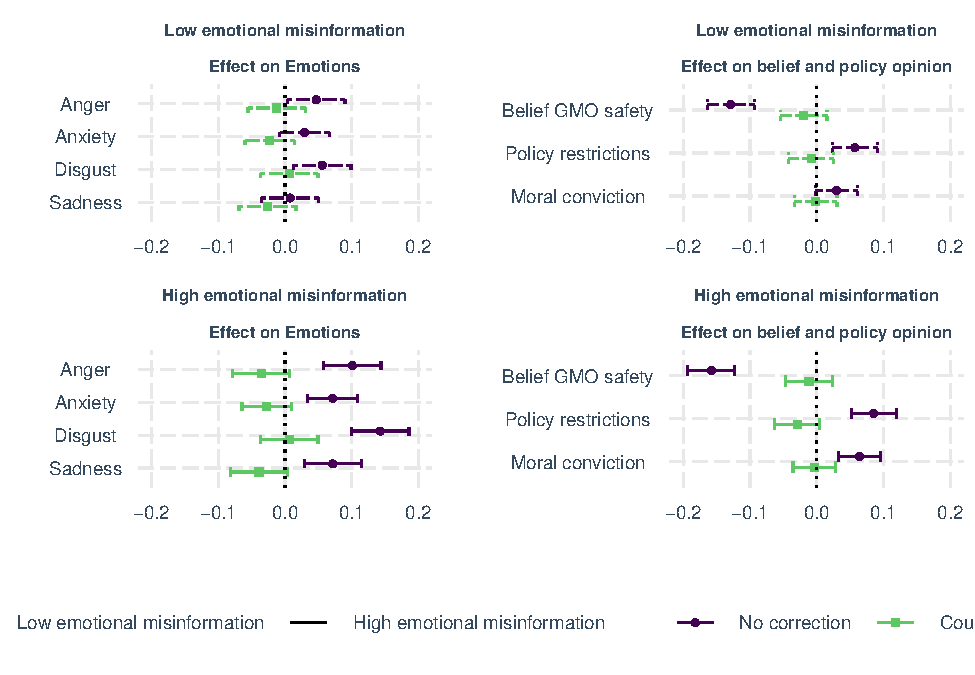
\includegraphics{paper_files/figure-latex/unnamed-chunk-6-2.pdf} 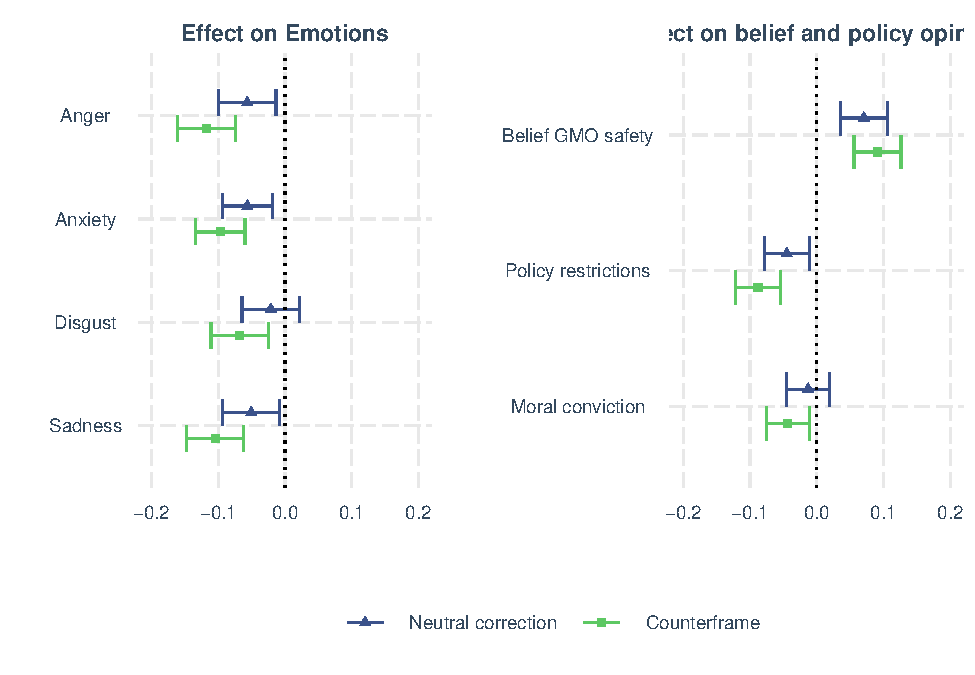
\includegraphics{paper_files/figure-latex/unnamed-chunk-6-3.pdf}

\hypertarget{conclusion}{%
\section{Conclusion}\label{conclusion}}

\newpage

\hypertarget{references}{%
\section{References}\label{references}}

\linespread{1}
\setlength{\parindent}{-0.2in}
\setlength{\leftskip}{0.2in}
\setlength{\parskip}{8pt}

\noindent

\hypertarget{refs}{}
\leavevmode\hypertarget{ref-bisgaard2019getting}{}%
Bisgaard, Martin. 2019. ``How Getting the Facts Right Can Fuel Partisan-Motivated Reasoning.'' \emph{American Journal of Political Science} 63(4): 824--839.

\leavevmode\hypertarget{ref-brady2017emotion}{}%
Brady, William J. et al. 2017. ``Emotion shapes the diffusion of moralized content in social networks.'' \emph{Proceedings of the National Academy of Sciences} 114(28): 7313--7318. \url{https://www.pnas.org/content/114/28/7313.short}.

\leavevmode\hypertarget{ref-chong2013counterframing}{}%
Chong, Dennis, and James N. Druckman. 2013. ``Counterframing effects.'' \emph{The Journal of Politics} 75(1): 1--16.

\leavevmode\hypertarget{ref-clifford2019emotional}{}%
Clifford, Scott. 2019. ``How Emotional Frames Moralize and Polarize Political Attitudes.'' \emph{Political Psychology} 40(1): 75--91. \url{https://onlinelibrary.wiley.com/doi/full/10.1111/pops.12507}.

\leavevmode\hypertarget{ref-diamond2020does}{}%
Diamond, Emily, Thomas Bernauer, and Frederick Mayer. 2020. ``Does providing scientific information affect climate change and GMO policy preferences of the mass public? Insights from survey experiments in Germany and the United States.'' \emph{Environmental Politics}: 1--20.

\leavevmode\hypertarget{ref-ecker2011terrorists}{}%
Ecker, Ullrich K. H., Stephan Lewandowsky, and Joe Apai. 2011. ``Terrorists brought down the plane!--No, actually it was a technical fault: processing corrections of emotive information.'' \emph{Quarterly journal of experimental psychology (2006)} 64(2): 283--310.

\leavevmode\hypertarget{ref-fernbach2019extreme}{}%
Fernbach, Philip M. et al. 2019. ``Extreme opponents of genetically modified foods know the least but think they know the most.'' \emph{Nature Human Behaviour} 3(3): 251--256.

\leavevmode\hypertarget{ref-flynn2017nature}{}%
Flynn, D. J., Brendan Nyhan, and Jason Reifler. 2017. ``The nature and origins of misperceptions: Understanding false and unsupported beliefs about politics.'' \emph{Political Psychology} 38: 127--150.

\leavevmode\hypertarget{ref-gaskell2010europeans}{}%
Gaskell, George et al. 2010. ``Europeans and Biotechnology in 2010. Winds of change?''

\leavevmode\hypertarget{ref-jerit2020political}{}%
Jerit, Jennifer, and Yangzi Zhao. 2020. ``Political misinformation.'' \emph{Annual Review of Political Science} 23: 77--94.

\leavevmode\hypertarget{ref-lazer2018science}{}%
Lazer, David M. J. et al. 2018. ``The science of fake news.'' \emph{Science} 359(6380): 1094--1096.

\leavevmode\hypertarget{ref-lewandowsky2012misinformation}{}%
Lewandowsky, Stephan et al. 2012. ``Misinformation and its correction: Continued influence and successful debiasing.'' \emph{Psychological Science in the Public Interest} 13(3): 106--131.

\leavevmode\hypertarget{ref-marcus2000affective}{}%
Marcus, George E., W. Russell Neuman, and Michael MacKuen. 2000. \emph{Affective intelligence and political judgment}. University of Chicago Press.

\leavevmode\hypertarget{ref-marcus2019applying}{}%
Marcus, George E. et al. 2019. ``Applying the theory of affective intelligence to support for authoritarian policies and parties.'' \emph{Political Psychology} 40: 109--139.

\leavevmode\hypertarget{ref-martel2020reliance}{}%
Martel, Cameron, Gordon Pennycook, and David G. Rand. 2020. ``Reliance on emotion promotes belief in fake news.'' \emph{Cognitive Research: Principles and Implications} 5(1): 47.

\leavevmode\hypertarget{ref-moors2013appraisal}{}%
Moors, Agnes et al. 2013. ``Appraisal theories of emotion: State of the art and future development.'' \emph{Emotion Review} 5(2): 119--124.

\leavevmode\hypertarget{ref-nyhan2019taking}{}%
Nyhan, Brendan et al. 2019. ``Taking fact-checks literally but not seriously? The effects of journalistic fact-checking on factual beliefs and candidate favorability.'' \emph{Political Behavior}: 1--22.

\leavevmode\hypertarget{ref-redlawsk2006feeling}{}%
Redlawsk, David. 2006. \emph{Feeling politics: Emotion in political information processing}. Springer.

\leavevmode\hypertarget{ref-roberts2018nobel}{}%
Roberts, Richard J. 2018. ``The Nobel Laureates' Campaign Supporting GMOs.'' \emph{Journal of Innovation \& Knowledge} 3(2): 61--65. \url{https://www.sciencedirect.com/science/article/pii/S2444569X18300064}.

\leavevmode\hypertarget{ref-rosenzweig2020misinformation}{}%
Rosenzweig, Leah et al. 2020. ``Misinformation and Emotions in Nigeria: The Case of COVID-19 Fake News.''

\leavevmode\hypertarget{ref-ryan2019actions}{}%
Ryan, Timothy J. 2019. ``Actions versus consequences in political arguments: Insights from moral psychology.'' \emph{The Journal of Politics} 81(2): 426--440.

\leavevmode\hypertarget{ref-ryan2017no}{}%
Ryan, Timothy J. 2017. ``No Compromise: Political Consequences of Moralized Attitudes.'' \emph{American Journal of Political Science} 61(2): 409--423.

\leavevmode\hypertarget{ref-ryan2014reconsidering}{}%
Ryan, Timothy J. 2014. ``Reconsidering moral issues in politics.'' \emph{The Journal of Politics} 76(2): 380--397.

\leavevmode\hypertarget{ref-sherman2002affective}{}%
Sherman, David K., and Heejung S. Kim. 2002. ``Affective perseverance: The resistance of affect to cognitive invalidation.'' \emph{Personality and Social Psychology Bulletin} 28(2): 224--237.

\leavevmode\hypertarget{ref-siegrist2020consumer}{}%
Siegrist, Michael, and Christina Hartmann. 2020. ``Consumer acceptance of novel food technologies.'' \emph{Nature Food} 1(6): 343--350.

\leavevmode\hypertarget{ref-skitka2020psychology}{}%
Skitka, Linda J. et al. 2020. ``The Psychology of Moral Conviction.'' \emph{Annual Review of Psychology} 72.

\leavevmode\hypertarget{ref-skitka2018attitude}{}%
Skitka, Linda J., Daniel C. Wisneski, and Mark J. Brandt. 2018. ``Attitude moralization: Probably not intuitive or rooted in perceptions of harm.'' \emph{Current Directions in Psychological Science} 27(1): 9--13.

\leavevmode\hypertarget{ref-swire2019they}{}%
Swire-Thompson, Briony et al. 2019. ``They Might Be a Liar But They're My Liar: Source Evaluation and the Prevalence of Misinformation.'' \emph{Political Psychology}.

\leavevmode\hypertarget{ref-thorson2016belief}{}%
Thorson, Emily. 2016. ``Belief Echoes: The Persistent Effects of Corrected Misinformation.'' \emph{Political Communication} 33(3): 460--480.

\leavevmode\hypertarget{ref-vosoughi2018spread}{}%
Vosoughi, Soroush, Deb Roy, and Sinan Aral. 2018. ``The spread of true and false news online.'' \emph{Science} 359(6380): 1146--1151.

\leavevmode\hypertarget{ref-walter2020fact}{}%
Walter, Nathan et al. 2020. ``Fact-Checking: A Meta-Analysis of What Works and for Whom.'' \emph{Political Communication} 37(3): 350--375.

\leavevmode\hypertarget{ref-wardle2017information}{}%
Wardle, Claire, and Hossein Derakhshan. 2017. ``Information Disorder: Toward an interdisciplinary framework for research and policy making.'' \emph{Council of Europe Report} 27.

\leavevmode\hypertarget{ref-weeks2015emotions}{}%
Weeks, Brian E. 2015. ``Emotions, Partisanship, and Misperceptions: How Anger and Anxiety Moderate the Effect of Partisan Bias on Susceptibility to Political Misinformation.'' \emph{Journal of Communication} 65(4): 699--719.

\leavevmode\hypertarget{ref-widmann2021how}{}%
Widmann, Tobias. 2021. ``How Emotional Are Populists Really? Factors Explaining Emotional Appeals in the Communication of Political Parties.'' \emph{Political Psychology} 42(1): 163--181.

\leavevmode\hypertarget{ref-wisneski2017moralization}{}%
Wisneski, Daniel C., and Linda J. Skitka. 2017. ``Moralization through moral shock: Exploring emotional antecedents to moral conviction.'' \emph{Personality and Social Psychology Bulletin} 43(2): 139--150.

\end{document}
